%!TeX spellcheck = en-ZA

\documentclass[11pt]{article}

\usepackage[utf8]{inputenc}
\usepackage[margin=1in]{geometry}
\usepackage[english]{babel}
\usepackage{tocloft}
\usepackage{amsmath}
\usepackage{amsfonts}
\usepackage{amssymb}
\usepackage[none]{hyphenat}
\usepackage{graphicx}
\usepackage{fancyhdr}
\usepackage{pdfpages}
\usepackage[font={small,it}]{caption}

\parindent 0ex
\linespread{1.5}
\setlength{\headheight}{30pt}
\setcounter{tocdepth}{1}
\pagestyle{fancy}

\fancyhead{}
%\fancyfoot{}
\fancyhead[L]{\slshape \MakeUppercase{Cryptogen User Manual}}
\rhead{
\includegraphics[width=1cm, height=1cm]{cryogen.png}
\includegraphics[width=1cm, height=1cm]{icon.png}}

\begin{document}
	%insert pdf cover page
	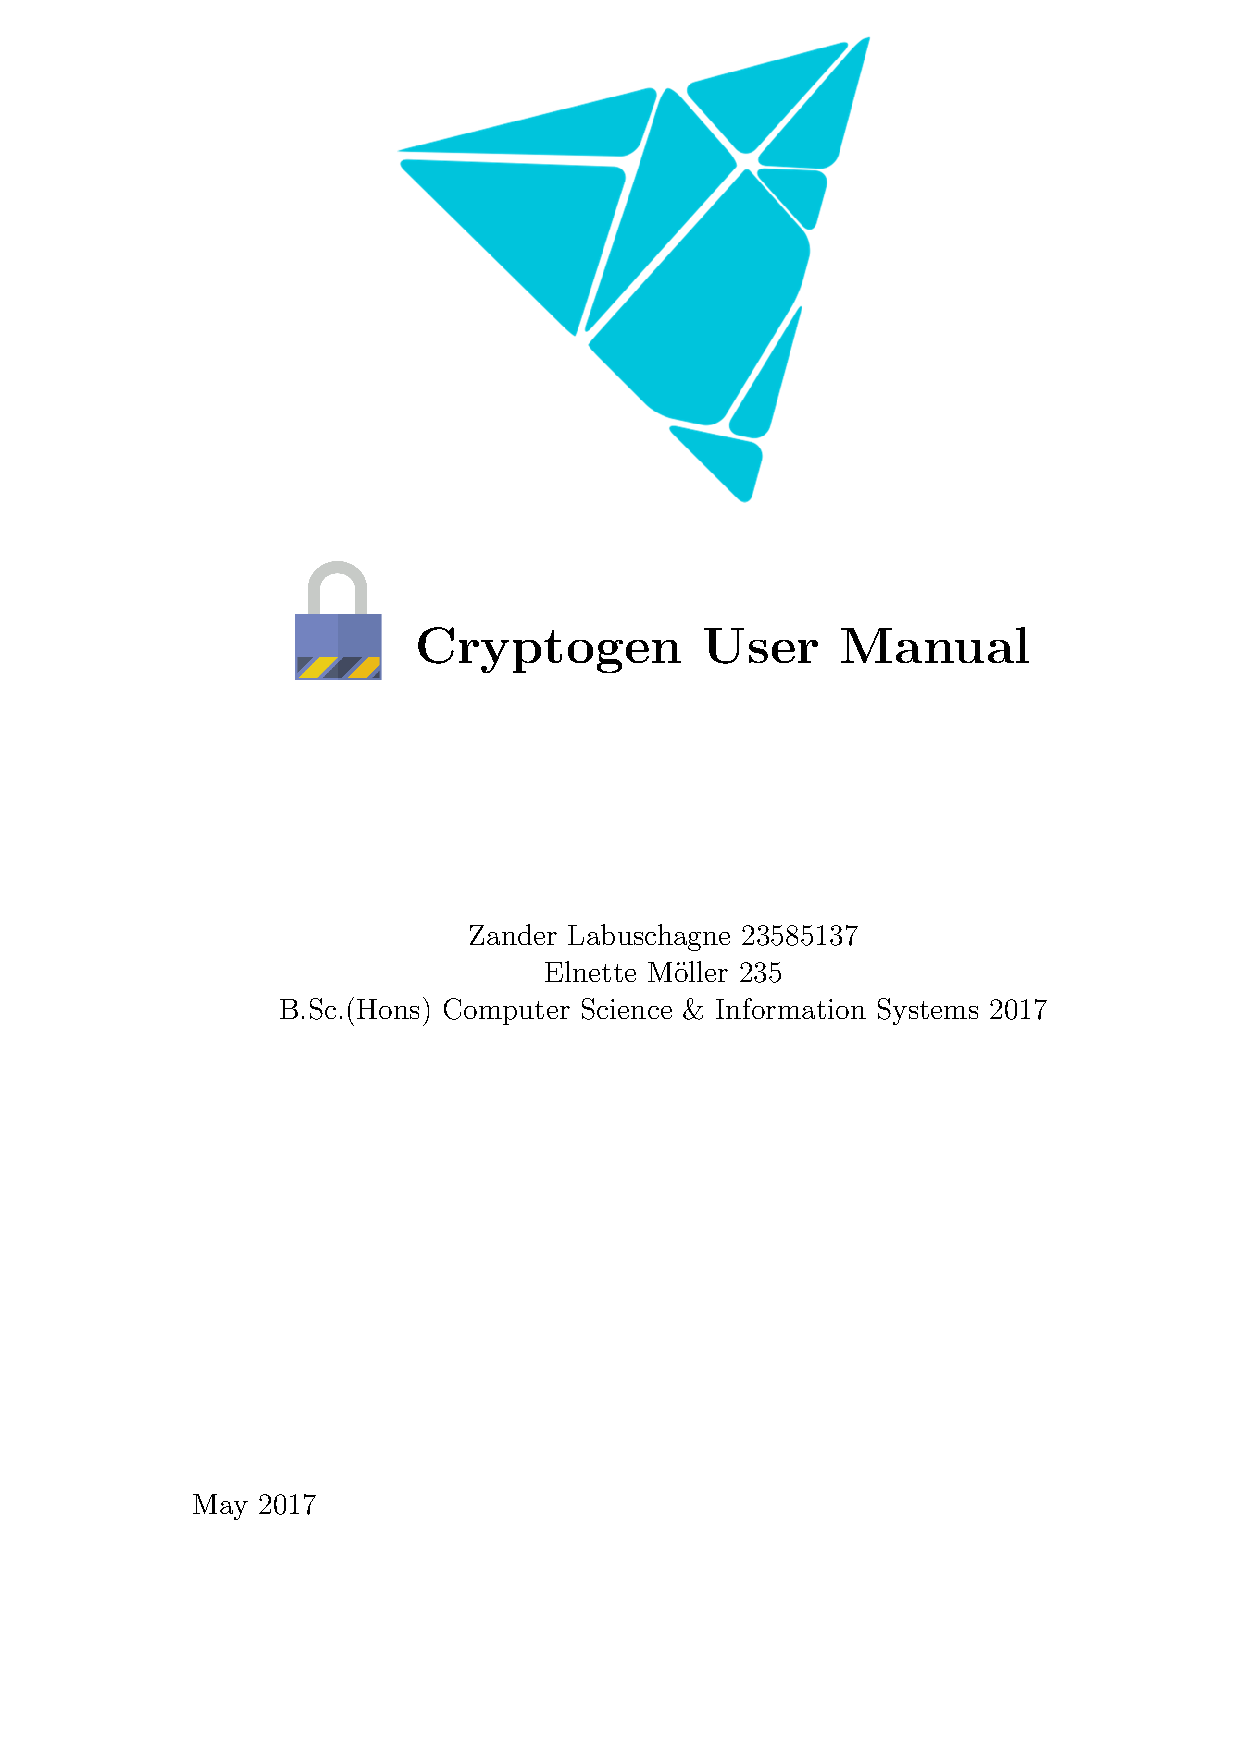
\includepdf[pages={-},offset=0mm 0mm, width=21.5cm, height=28cm]{Cover.pdf}

    \renewcommand{\cftsecleader}{\cftdotfill{\cftdotsep}} % TOC Dotted Lines
    \tableofcontents
    \thispagestyle{empty}
    \clearpage

	%\printglossary[title=Abbreviation]

    \setcounter{page}{1}

	\section{Introduction}
	\subsection{Intended Readership}
	This documented is intended for the users of the Cryptogen application used for the encryption and decryption of messages and files which is developed by two computer science students at the Nort-West University, Zander Labuschagne \& Elnette M\"{o}ller.

	\subsection{Applicability}
	This user manual only applies to version 1.x of the Cryptogen application developed by Zander Labuschagne \& Elnette M\"{o}ller.

	\subsection{Purpose}
	The purpose of this document is to aid the users of the Cryptogen application so they can use it properly and as intended by the developers. This document hopes to clarify any misunderstandings its users might have.

	\subsection{Motivation \& Background}
	Cryptogen is developed as part of the Computer Security module for B.Sc. Computer Science \& Information Systems Honnors students at the North-West University, Potchefstroom Campus. The goal of this project was to provide students with experience in elementary cryptosystems by developing a small system which implements different encryption algorithms. It was expected of one to two student to work together and develop an application which satisfies the following requirements:
	\begin{itemize}
		\item Handle encryption and decryption of messages and files.
		\item Graphical interface to simplify the functioning.
		\item Any programming language(s) may be used.
		\item The following algorithms had to be implemented:
		\begin{itemize}
			\item Vigen\`{e}re Cipher
			\item Vernam Cipher
			\item Columnar Transposition Cipher
			\item Own implementation
		\end{itemize}
	\end{itemize}

	\section{User Guide}
	\subsection{Support}
	\subsubsection{Linux}
	This project was partly developed on a GNU/Linux system, more specifically Manjaro ArchLinux 17.01 KDE x86\_64 running Manjaro kernel version 4.11. Linux systems are fully supported and Cryptogen is expected to run flawless on these systems, but is not guaranteed. Any bugs and inconsistencies may be reported to the developers, at least one of the developers aims to maintain this project for UNIX-like systems.

	\subsubsection{Windows}
	This project was partly developed on a Windows platform, thus some Windows support is provided such as a GUI specifically adapted for Windows. Many problems or inconsistencies were experienced by the developers when the application was used on a Windows platform such as malfunctioning drag \'n drop, so there is no guarantee that the application will function proporly on Windows systems. It is very complicated to create an installer or portable .exe for Windows from a .jar executable and the little third party software that exists to make this process simpler is very expensive hence no Windows executable or intsaller. There is no guaratee that the developers will address any bugs or problems experienced on Windows systems but feedback is welcome just to keep record of what functions well.

	\subsubsection{macOS}
	This application was not yet tested on a macOS system and since the lack of a macOS system from the developers no dedicated installer or macOS executable(.app or .dmg) was made. However at least one of the two developers aims add support for macOS systems in the future. Since a Java .jar file is provided one can run the .jar executable on a macOS system if Java Runtime Environment 1.8 or higher is installed. To be able to read this document a PDF reader is required such as Skim.

    	\section{Reflection}
		...

    \newpage
    \bibliographystyle{plain}
    \bibliography{ref}
    \addcontentsline{toc}{section}{{}References}
    \thispagestyle{plain}
    \clearpage

  %  \section*{Appendix A: Research Proposal}
  %  \addcontentsline{toc}{section}{{}Appendix A: Research Proposal}
    %\pagenumbering{gobble}
  %  \includepdf[pages={-},offset=0mm 0mm, width=21.5cm, height=28cm]{Appendix_A.pdf}

\end{document}
